\section{Polarimetric products (POL)}
\label{sec:pol}

The \acs{pol} \acs{ard} products considered in this project correspond to the polarimetric covariance matrix, which can be provided in radar coordinates (\acs{cov}) or in geographical coordinates (\acs{gcov}), i.e. after geocoding. The inputs required to generate these products correspond to individual \acs{slc} images or to previously generated \acs{cslc} products. In both cases, the processing required to compute each entry of the matrix is totally equivalent to what is done to produce \acs{nrb} data, so the reader is referred to \autoref{sec:nrb} for consulting the models and computational performance involved in such a product.

Since the \acs{pol} products involve more than one input polarimetric channel, the extension of the processing from \acs{nrb} to \acs{pol} must comply with the following rules:
\begin{itemize}
    \item When the input data is in \acs{cslc} form, the same co-registration grid (offsets of the secondary images with respect to the primary image) and interpolation must have been applied to all polarimetric channels. The common rule consists in computing the co-registration grid using only one channel (usually a co-polar one, i.e. VV or HH), and then applying it to all channels available.
    \item The same processing, i.e. the same algorithms, options and parameters (e.g. size of kernel), must be used for computing all entries of the matrix.
    \item Any spatial filtering or multi-look should be applied in radar coordinates, i.e. before geocoding, for preserving all the polarimetric information.
    \item The diagonal entries of the covariance matrix correspond to the backscattering coefficient of the individual polarimetric channels, and thus they are positive real numbers. However, the off-diagonal elements of the matrix are formed as products of the \acs{slc} values of different channels and, thus, they are complex values. Therefore, the implementation must take into account this difference in the type of data. 
\end{itemize}

In addition, the \acs{nrb} products are usually generated with a small equivalent number of looks (\acs{enl}) because they aim at preserving as much spatial resolution as possible. However, due to the higher dimensionality of the covariance matrix, the \acs{enl} required to properly estimate the covariance matrix is much larger than in the \acs{nrb} case. Because of that, an additional spatial filtering or multi-look is usually applied, hence changing the workflow with respect to a conventional \acs{nrb}. In fact, this is the main reason for providing also the \acs{cov} product, as the end user will be able to apply the spatial filtering required in radar coordinates. The \acs{cov} product will include a layer with a look-up table, or equivalent information, to geocode the result of the spatial filter, i.e. to transform it into a \acs{gcov} product, which is directly usable as an \acs{ard}.

\subsection{Evaluation criteria}
\label{sec:pol_criteria}

Apart from the impact of the spatial filtering or multi-looking, the conversion from a \acs{slc} or \acs{cslc} product to a \acs{pol} product does not entail any difference with respect to the conversion to \acs{nrb}. In other words, the generation of a \acs{pol} product must be evaluated in the same way as the generation of \acs{nrb}.

In order to stress the relevance of the equivalent number of looks (\acs{enl}) in the polarimetric case, which is more demanding than the single-pol case, in this section we illustrate the \acs{enl} provided by the different processing strategies, and its impact on polarimetric features derived from the resulting products.

\autoref{fig:pol_enl} shows the empirical estimates of \acs{enl} for two processing approaches: without multi-looking or spatial filtering (denoted as Shiroma), and with multi-looking for different window sizes (azimuth $\times$ range). The estimation of ENL from the output image is computed using the following expression~\cite{lee_intensity_1994}:
\begin{equation}
\text{ENL} = \frac{\hat{I}^2}{\sigma_I^2}
\end{equation}
where $\hat{I}$ and $\sigma_I^2$ denote the mean and the variance, respectively, of an intensity image (i.e. backscattering coefficient).
For this purpose, a homogeneous area on the scene is selected, which in this case corresponds to the sea.

\begin{figure}[ht!]
\centering
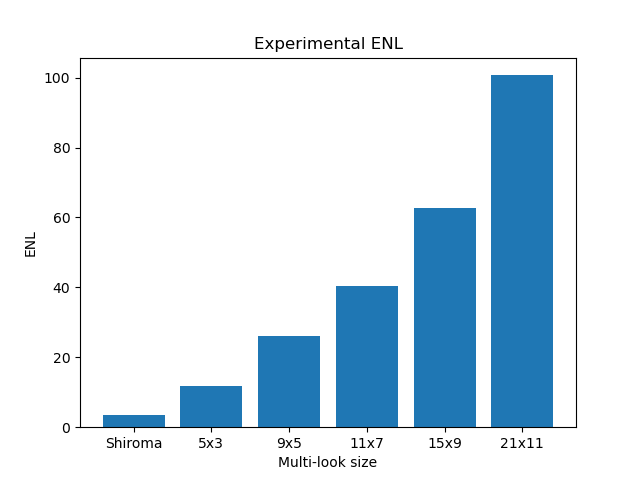
\includegraphics[width=0.8\textwidth]{Figures/pol/pol_enl_vs_multilook.png}
\caption{Equivalent number of looks (\acs{enl}) for two processing strategies: without multi-looking (denoted as Shiroma) and with multi-look for a set of window sizes (azimuth $\times$ range). Measurements are carried out with a dual-pol stripmap SAOCOM image over Naples (DSC pass, S4 beam) acquired on 28-02-2021. \acs{enl} is estimated empirically over a homogeneous area on the sea.}
\label{fig:pol_enl}
\end{figure}

The values shown in \autoref{fig:pol_enl} demonstrate that, due to the typical oversampling of \acs{sar} images, the number of looks is much smaller than the number of samples employed to compute averages in the multi-looking. In addition, it must be noted that the \acs{enl} value provided without multi-look, i.e. using only the geocoding step defined in~\cite{Shiroma2022}, is just 3.5 over this flat area. The \acs{enl} value in slopes facing the radar is much smaller, hence compromising the statistical significance of measures derived from the polarimetric covariance matrix.  

To assess the impact of the available \acs{enl} upon parameters derived from the \acs{pol} products, we show here the polarimetric entropy, which is widely used for scene characterisation and classification~\cite{Hajnsek2021}. 
For dual-pol data, polarimetric entropy $H$ is defined as:
\begin{equation}
    H = - \sum_{i=1}^2 p_i \cdot \log_2 p_i
\end{equation}
where
\begin{equation}
    p_i = \frac{\lambda_i}{\lambda_1 + \lambda_2},
\end{equation}
and $\lambda_1$ and $\lambda_2$ are the two eigenvalues of the dual-pol covariance matrix. A low entropy (close to 0) denotes the presence of a dominant scattering mechanism, whereas a high value (close to 1) represents a non-defined polarimetric response from the scene.

\autoref{fig:pol_entropy} shows the images of dual-pol entropy computed from the \acs{gcov} products pre-processed using Shiroma's approach and two different multi-look sizes. Entropy is generally low over the sea surface because its backscatter is dominated by a surface component, whereas it is very high over forested areas. Notably, there is a extremely high entropy zone in the lower left corner of the image, which corresponds to very calm water close to Ischia island. In this region the backscattering level is very close to the noise level, and hence the very high entropy. 

\begin{figure}[ht!]
\centering
\begin{tabular}{cc}
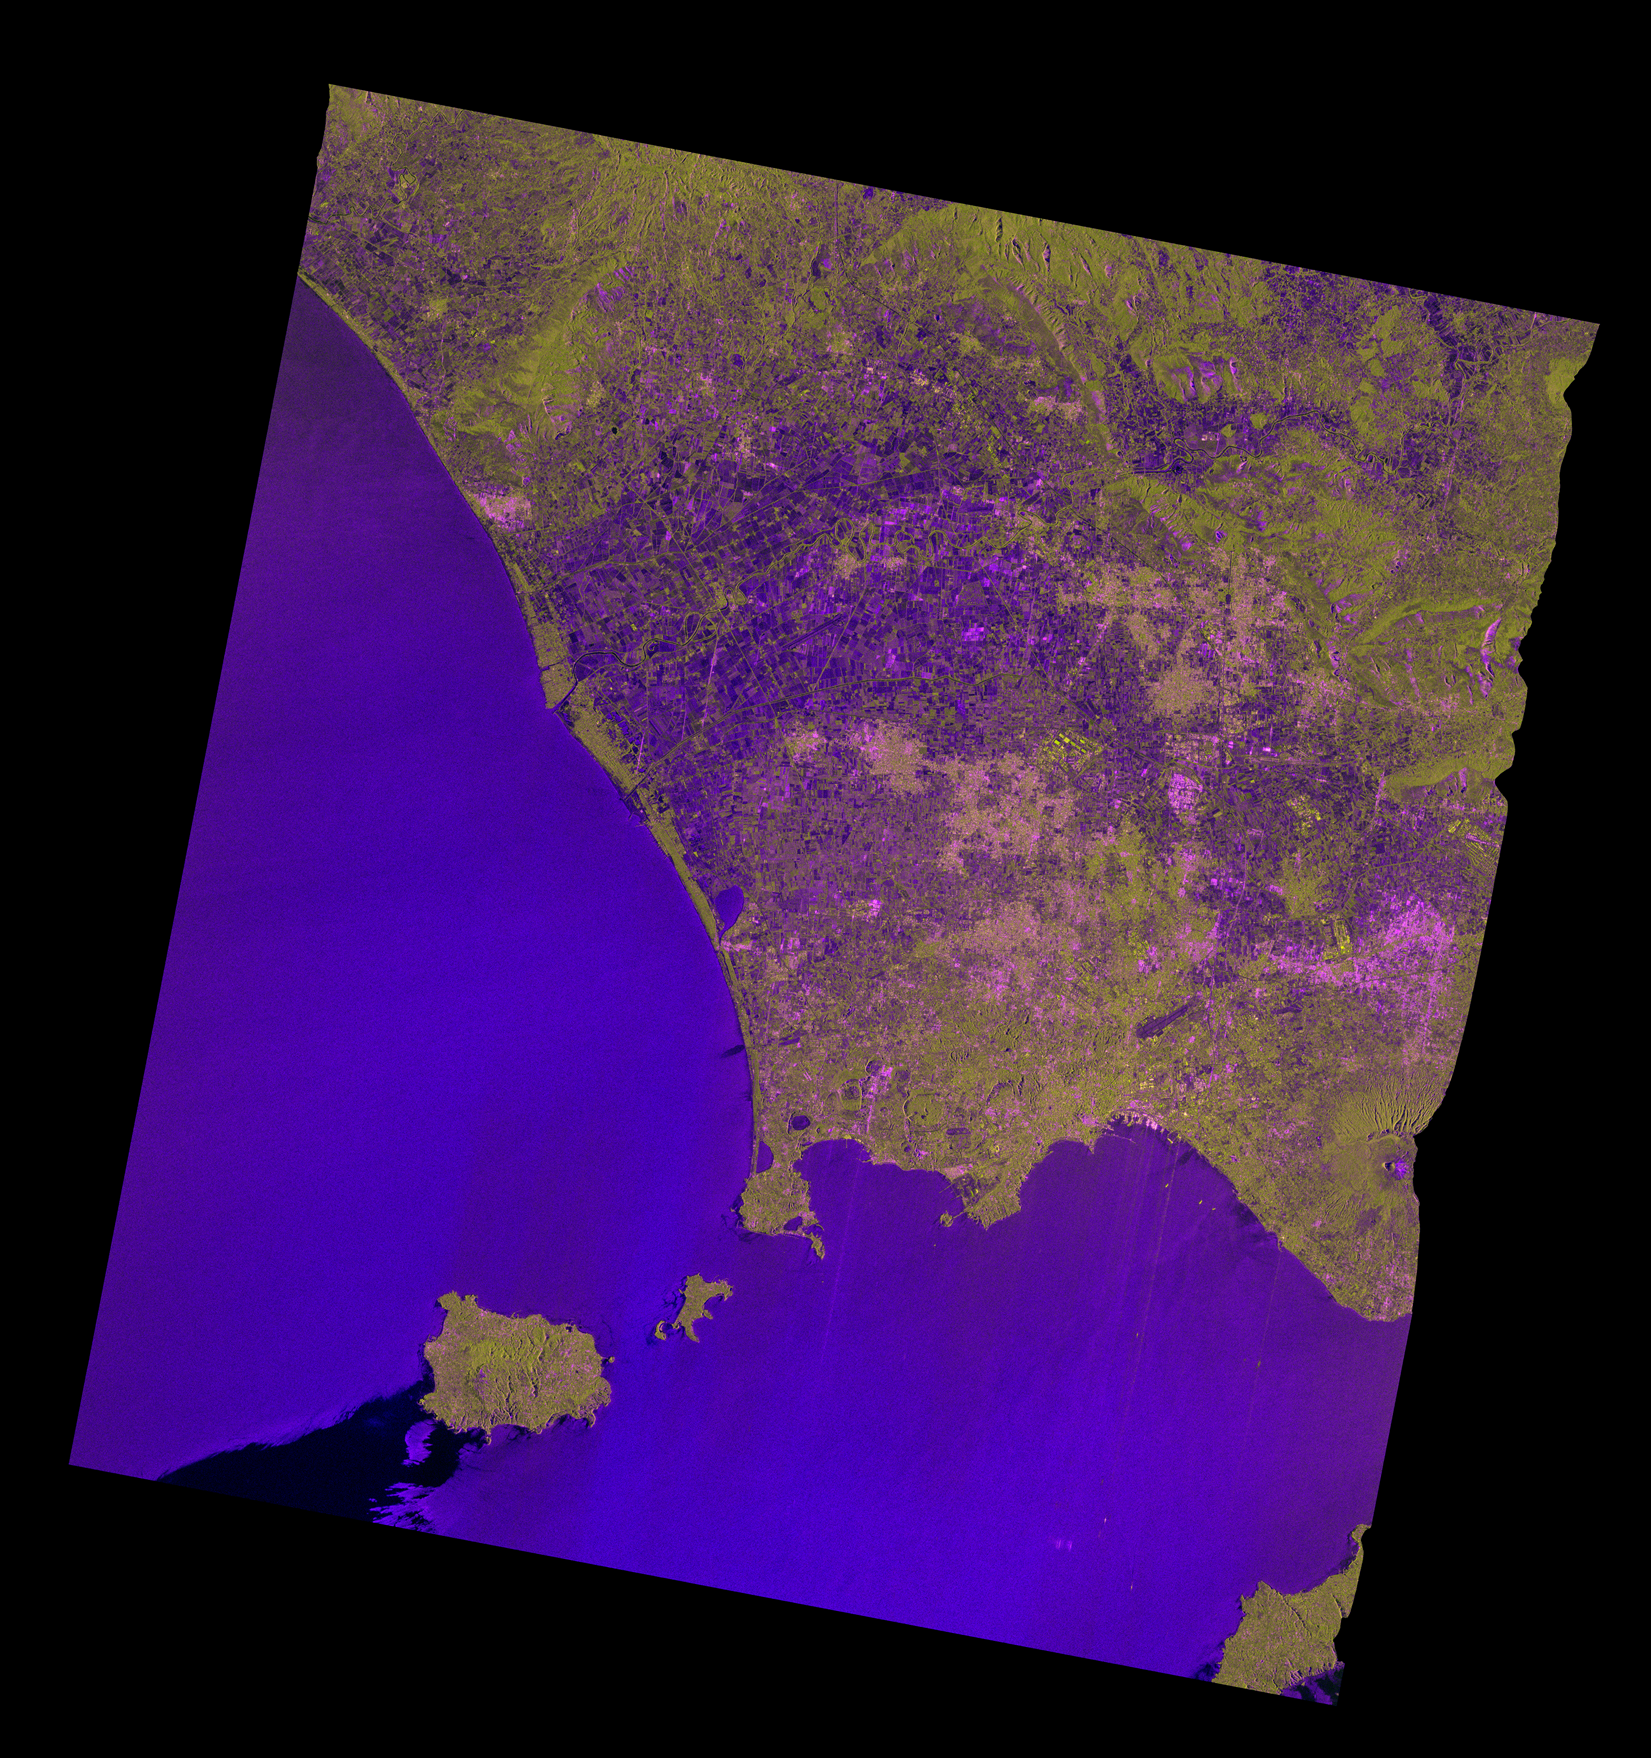
\includegraphics[width=0.35\textwidth]{Figures/pol/GCOV_LinearRGB_lowres.png}
 & 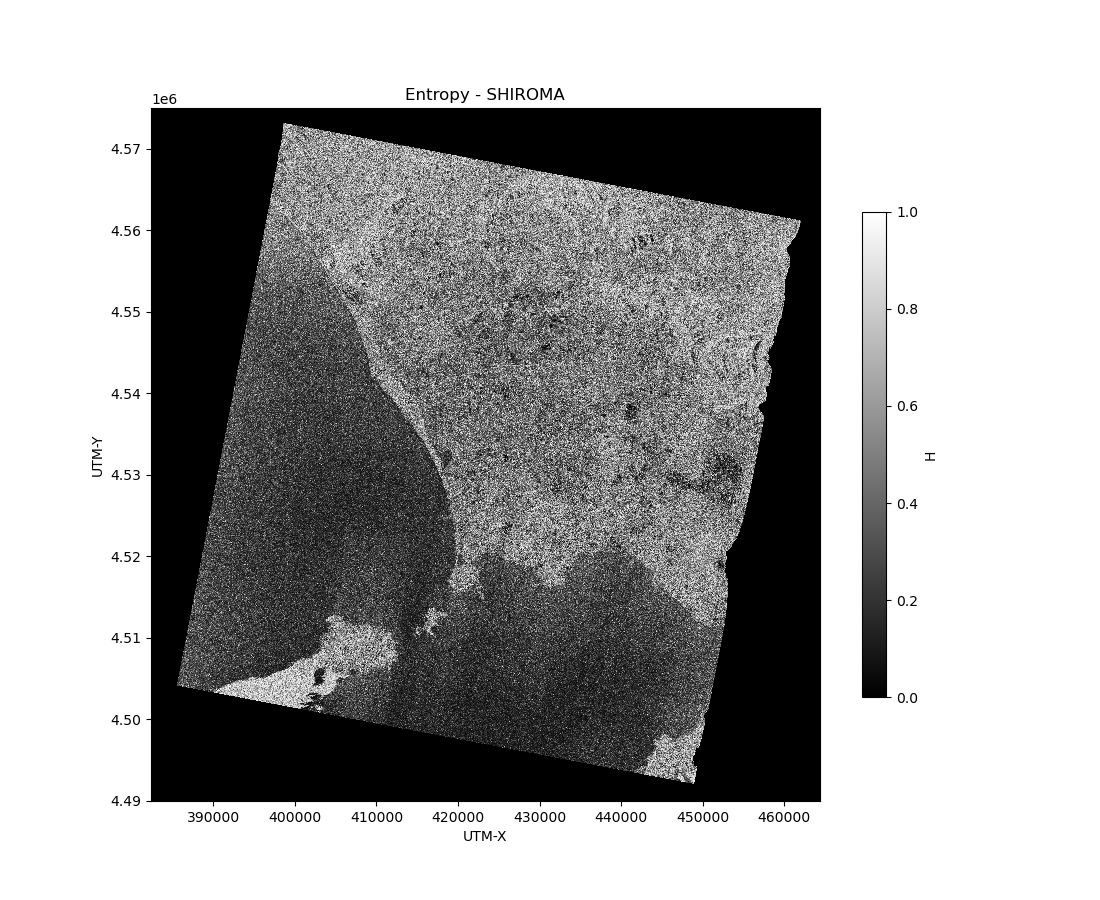
\includegraphics[width=0.5\textwidth]{Figures/pol/H_Shiroma.png}
 \\
(a) & (b) \\
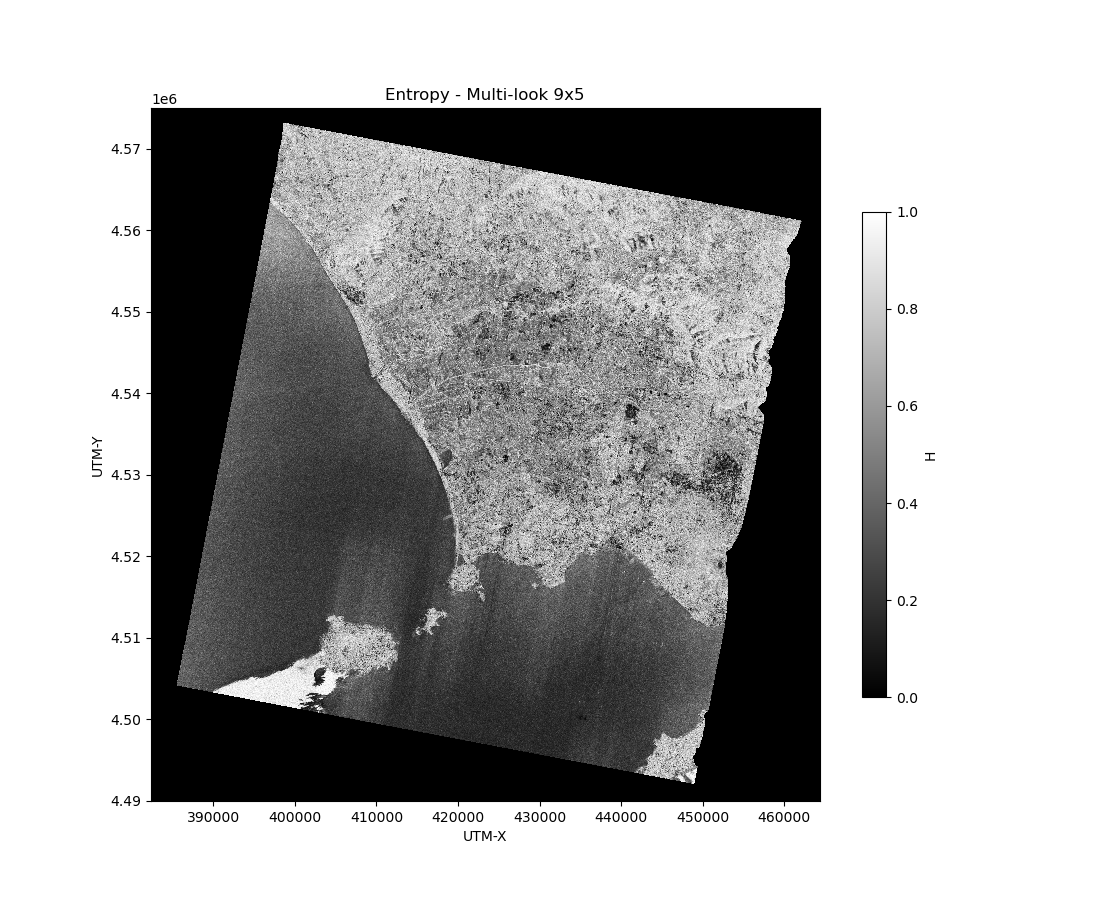
\includegraphics[width=0.5\textwidth]{Figures/pol/H_9x5.png}
 & 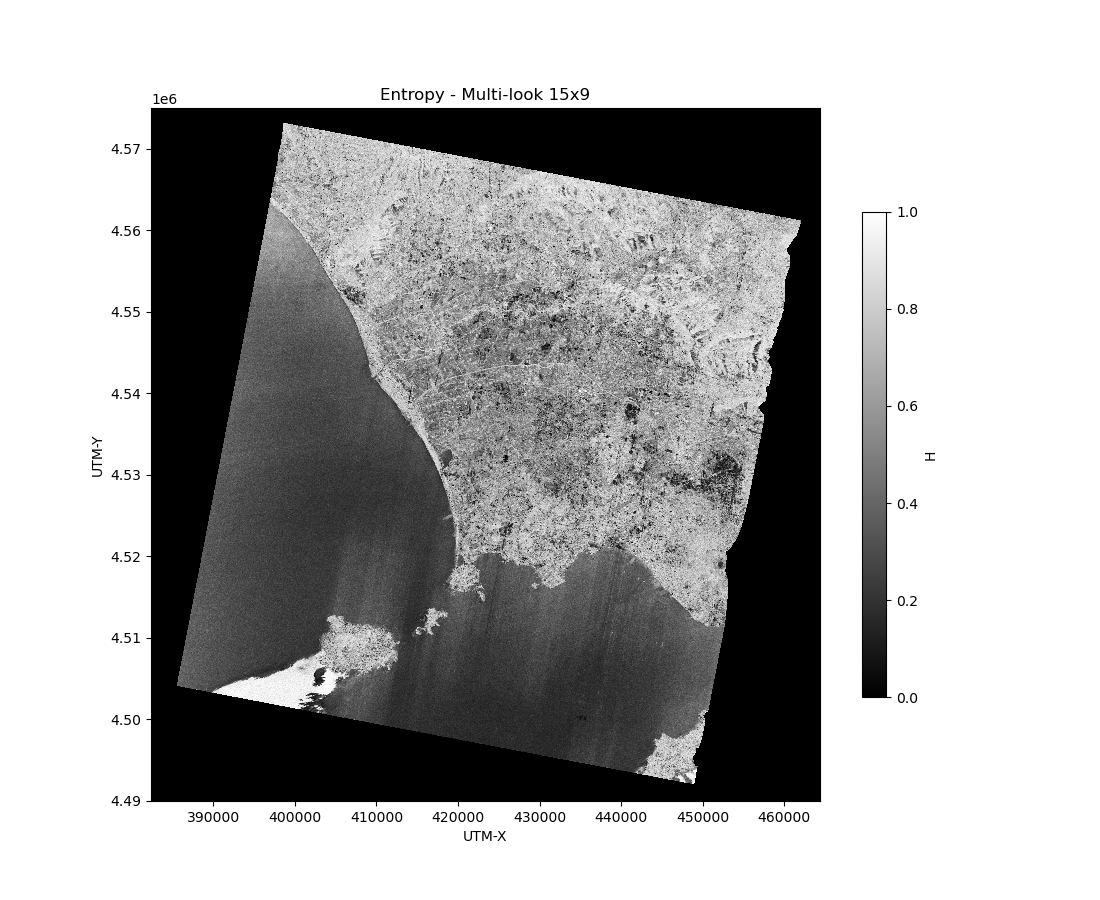
\includegraphics[width=0.5\textwidth]{Figures/pol/H_15x9.png}
 \\
(c) & (d)
\end{tabular}
\caption{Comparison of the dual-pol entropy computed for various processing options, using a dual-pol stripmap SAOCOM image over Naples (DSC pass, S4 beam) acquired on 28-02-2021. The RGB false colour composite is shown in (a). Images of entropy derived from the data pre-processed using: (b) Shiroma's approach, (c) 9x5 Multi-look, and (d) 15x9 Multi-look. }
\label{fig:pol_entropy}
\end{figure}

The computation of entropy from the sampled covariance matrix is known to be underestimated, being the bias more pronounced for higher entropies and for lower values \acs{enl}~\cite{LopezMartinez2005}. As a result, the measured entropy in this scene when no multi-look is applied (\autoref{fig:pol_entropy}b, \acs{enl} = 3.5) is clearly lower than in the multi-look cases (\autoref{fig:pol_entropy}c and \autoref{fig:pol_entropy}d).

\autoref{tab:pol_enl_H} shows the mean entropy measured at different locations of the scene for the same three processing options used in \autoref{fig:pol_entropy}. The small \acs{enl} provided by the approach without multi-look has a clear impact on the estimation of entropy when it is very high, namely over calm water and in forest areas, but also in an agricultural zone characterised by a moderately low entropy. 

\begin{longtblr}[
	label = tab:pol_enl_H,
	entry = none,
	caption = {Mean dual-pol entropy for different processing cases at various land cover areas},
	]{
		width = \linewidth,
		colspec = {Q[l,20]Q[c,20]Q[c,20]Q[c,20]},
		hlines,
		hline{1-Z} = {-}{0.05em},
	}
	\textbf{Zone}   & \textbf{Shiroma}   & \textbf{9x5 Multi-look} & \textbf{15x9 Multi-look} \\
	Sea & 0.23 & 0.26 & 0.26 \\
    Calm water & 0.74 & 0.92 & 0.95 \\
    Forest & 0.68 & 0.81 & 0.83 \\
    Urban & 0.29 & 0.30 & 0.30 \\
    Crops & 0.40 & 0.47 & 0.48 \\
\end{longtblr}



%Impact of asc/dsc and order of steps.


\subsection{Theoretical models}
\label{sec:pol_models}


The formation of the \acs{pol} products from the input \acs{slc} images consists of three or four steps:
\begin{enumerate}
\item Terrain flattening correction (also known as RTC), which can be directly applied to the images in \acs{slc} format.
\item Generation of the complex cross-products between polarimetric channels (off-diagonal elements of the covariance matrix), and the real intensity values of each channel (diagonal elements of the covariance matrix).
\item Spatial filtering or multi-looking of every matrix entry.
\item Geocoding of all matrix entries, which is required to produce a \acs{gcov}. 
\end{enumerate}

As previously explained, the approach defined for the NISAR \acs{gcov} product~\cite{NISAR_GCOV_ProdSpec} performs the last two steps simultaneously. In that case, the extent of the spatial filter depends on the relationship between the size of the output product (posting) and the corresponding pixels in the \acs{slc} image, which differs over the image due to topographic slopes.

If a \acs{cov} product is to be produced, i.e. without geocoding, the spatial filtering step is mandatory to 
estimate a true covariance matrix.

The definition of the $C_3$ matrix to be employed in the quad-pol case is the following one, denoted as $C_{3mod}$ in~\cite{CEOS-ARD_PFS_POLSAR}:
\begin{equation}
    C_{3mod} =
    \begin{bmatrix}
    <|HH|^2>         &  <HH  \cdot HV^*> &    <HH  \cdot VV^*> \\
    <HV  \cdot HH^*> &  <|HV|^2>         &    <HV  \cdot VV^*> \\
    <VV  \cdot HH^*> &  <VV  \cdot HV^*> &     <|VV|^2>
    \end{bmatrix} \label{eq:C3mod}
\end{equation}
where the brackets denote the estimation step (i.e., spatial filtering or multi-look). In principle, the cross-polar channel HV is assumed to be equal to VH due to reciprocity, but this aspect can be forced using a symmetrization (explained later in this section).

It is to be noted that the entries of the diagonal correspond to the \acs{nrb} of the individual polarimetric channels. 

The definition in \eqref{eq:C3mod} does not correspond to the standard polarimetric covariance matrix (shown in \eqref{eq:C3}), because some constant factors are not present. Therefore, any user employing data in the proposed form \eqref{eq:C3mod} must take into account the conversion to the standard form \eqref{eq:C3} if it is required by the post-processing to be applied (e.g. target decompositions).

\begin{equation}
    C_{3} =
    \begin{bmatrix}
    <|HH|^2>               & \sqrt 2 <HH \cdot HV^*> & <HH  \cdot VV^*> \\
    \sqrt 2 <HV\cdot HH^*> & 2 <|HV|^2>              & \sqrt 2 <HV\cdot VV^*> \\
    <VV HH^*>              & \sqrt 2 <VV \cdot HV^*> &     <|VV|^2>
    \end{bmatrix} \label{eq:C3}
\end{equation}

 In the case of quad-pol data, due to reciprocity, and after an adequate calibration, the two cross-polar channels (HV and VH) should be equal and are only different due to the presence of noise. Because of that, for the definition of the covariance matrix (\eqref{eq:C3mod} and \eqref{eq:C3}), only three channels are considered, i.e. HH, VV and one cross-polar channel (HV or VH). 

A common practice, also considered in the definition of the \acs{gcov}-NISAR product~\cite{NISAR_GCOV_ProdSpec}, consists in averaging the two cross-polar channels and using the resulting average in the construction of the covariance matrix in the \acs{ard} product. This operation is called symmetrization in the polarimetric literature.

Regarding the dual-pol mode with linear polarisations, the $C_2$ covariance matrix is defined as follows:
\begin{equation}
C_{2} =
    \begin{bmatrix}
    <|VV|^2>       & <VV \cdot VH^*> \\
    <VH\cdot VV^*> & <|VH|^2>
    \end{bmatrix} \label{eq:C2vh}
\end{equation}

A similar expression could be obtained by transmitting a horizontal polarisation, or even a circular polarisation, as it it done in compact- or hybrid-pol modes (see D1~\cite{D1} for more details).

Provided that the covariance matrices are Hermitian, only the off-diagonal elements of the upper-triangular matrix are saved as product layers. The lower-triangular elements are just complex conjugated of the upper-triangular ones. As a result, 3 layers are saved in the dual-pol case, and 6 layers are saved in the quad-pol case.

\subsection{Computational performance}
\label{sec:pol_computation}

The computational burden of generating \acs{pol} products is equivalent to the one of a \acs{nrb} product, but more layers are generated.

The \acs{rtc} is applied to the \acs{slc} images of each channel. So the computational burden of this step is the one of \acs{nrb} multiplied by the number of channels: 2 for dual-pol, and 4 for quad-pol (or 3 if the symmetrization is computed before the correction) . It must be noted that the same coefficients are applied to all channels, so the computation of the coefficients, which is the most demanding operation, has the same burden as \acs{nrb}.

As for the symmetrization, which consists of a simple arithmetic mean of two images, its computational burden is very small.

Regarding the computation of the output layers (entries of the covariance matrix), the processing time is also the same of this step for \acs{nrb} but multiplied by the number of output layers, i.e., 3 layers for dual-pol case, and 6 layers for the quad-pol case.



\subsection{Criticalities and weaknesses}
\label{sec:pol_criticalities}

Any test of the polarimetric quality of the \acs{pol} products depends on the quality of the \acs{slc} data, especially regarding the radiometric calibration and other phase-related effects, such as Faraday rotation. 
Consequently, any analysis of the quality of the products (from the polarimetric point of view) relies on the input data, and not on the generation algorithm itself.

In this sense, there exists some basic tests of the polarimetric calibration of the data that could be applied, but all of them are designed for quad-pol data, not for dual-pol data.

% Preliminary analysis on FR

Regarding Faraday rotation (\acs{fr}), a preliminary analysis on the impact it will have on the \acs{pol} products derived from \acs{rosel} is included in the following section.

\subsubsection{Impact of Faraday Rotation on POL products}
\label{sec:pol_fr}

%Considering that in ROSE-L it will not be possible to correct for the Faraday rotation it is kindly requested to elaborate a little bit more this point to provide some practical indicatioon about  what is the amount of residual faraday rotation that can be afforded without impairing completely the product 

The impact of \acs{fr} on the polarisation of the electromagnetic waves is well-known and is properly described in the literature~\citep{Wright2003,Freeman2004a,Freeman2004b}, as there exists a sound physical model to analyse it. \acs{fr} depends on the value of \acs{tec}, and hence its influence changes as a function of time (within the day and along the year) and space (geographical coordinates, especially latitude). 

The parameter that represents the impact on the wave is the \emph{one-way rotation angle}, whose absolute value ranges from very low values, close to zero, to more than 20 degrees in very extreme cases at L-band~\citep{Meyer2008}. 

The effect of \acs{fr} is conceptually similar to cross-talk, i.e. polarimetric channels interfere (are partially added) to each other.

With quad-pol data, \acs{fr} can be estimated and fully corrected by exploiting reciprocity~\citep{Bickle1965,Wright2003,Freeman2004b,Meyer2008}.

However, with dual-pol data, the correction requires: 1) the \acs{tec} value (which can be retrieved from auxiliary measures, as for \acs{etad}) and 2) the knowledge of the actual scattering matrix of the scene (which is not known). Consequently, the only way to try to correct \acs{fr} consists in assuming some scattering properties of the scene and using them (with the \acs{tec} external information) to apply the correction. As a result, the correction performance depends on the validity of the assumptions.

The effect of \acs{fr} increases with increasing contrast between the scattering matrix elements. In other words, the more different are the backscattering coefficients at the co- and cross-polar channels (e.g., VV and VH), the stronger the effect of FR. For instance, at L-band, bare surfaces are characterised by a very low cross-pol component, so they are more impacted than forests (characterised by a high cross-pol return, close to the co-polar channel value).

The co-polar (HH and VV) channels suffer only some tenths of dB of decrease with respect to their true value (less than 0.1~dB of decrease for 80\% of the expected \acs{fr} levels~\citep{Hajnsek2019}. The behavior of the cross-pol channels is more dynamic and changes depending on the scene and the \acs{fr} angle (it can reach a 4~dB increase in some situations). This means that the \acs{nrb} products (just backscattered intensity) are also affected by \acs{fr}, especially the cross-polar channel~\citep{Freeman2004a}.

Regarding the complex correlation between the co- and the cross-polar channel (e.g. VV and VH) it is normally very low (null in theory) over reflection-symmetric scenes (in practice, all but urban areas, infrastructures, and slopes). However, in presence of \acs{fr}, the influence of one channel upon the other increases this correlation. Once again, it could be approximately corrected under the assumption of knowledge of the underlying correlation.

\autoref{fig:pol_fr_dualpol_baresoil} and \autoref{fig:pol_fr_dualpol_forest} show the impact of \acs{fr} without any correction over ‘bare soil’ and ‘upland forest’ classes, for which the scene parameters defined in \citep{Freeman2004b}) are used.

\begin{figure}[h!]
\centering
\begin{tabular}{ccc}
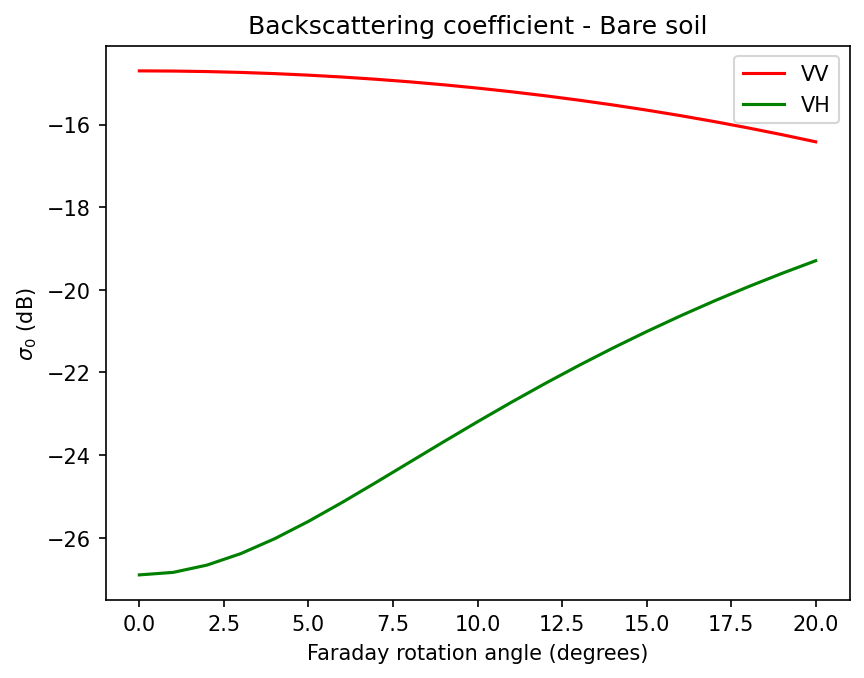
\includegraphics[width=0.32\textwidth]{Figures/pol/FR_bacskcatter_Bare soil.png}
 & 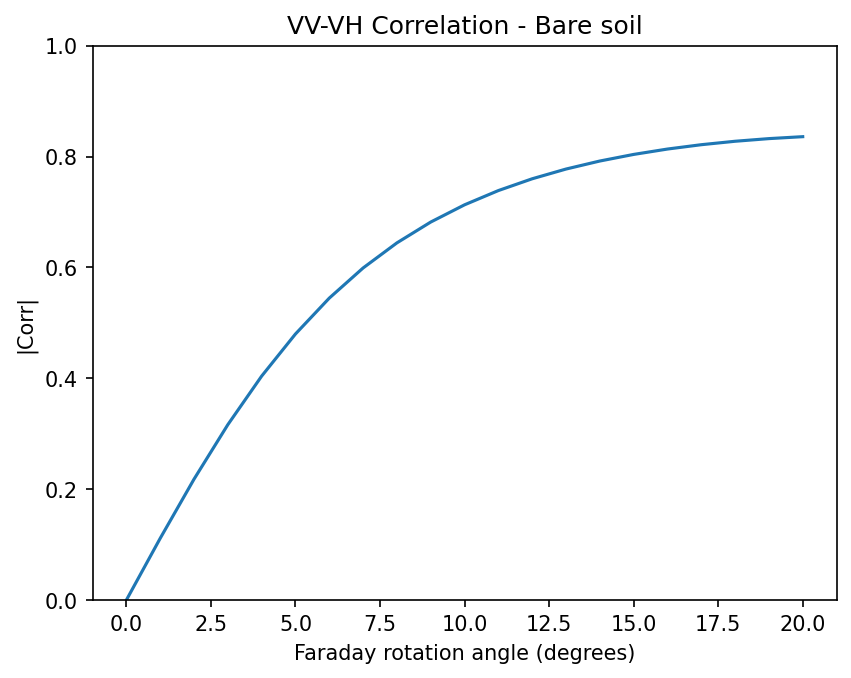
\includegraphics[width=0.32\textwidth]{Figures/pol/FR_VV-VH_Correlation_Bare soil.png}
 &
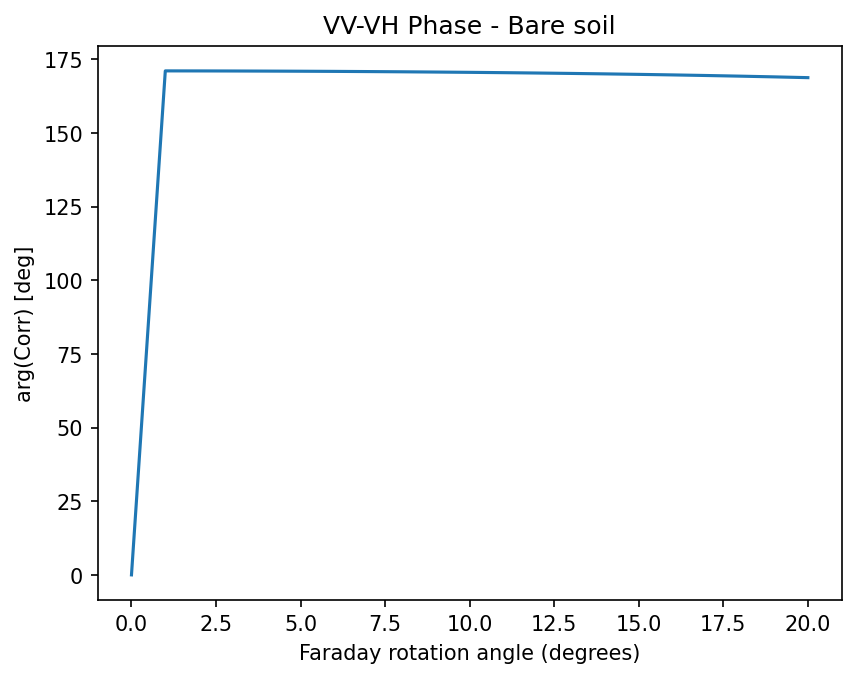
\includegraphics[width=0.32\textwidth]{Figures/pol/FR_VV-VH_Phase_Bare soil.png} \\
(a) & (b) &
(c) 
\end{tabular}
\caption{Effect of \acs{fr} upon the dual-pol response of bare soil. (a) Backscattering coefficients, (b) Correlation between channels, (c) Phase between channels.}
\label{fig:pol_fr_dualpol_baresoil}
\end{figure}
\begin{figure}[h!]
\centering
\begin{tabular}{ccc}
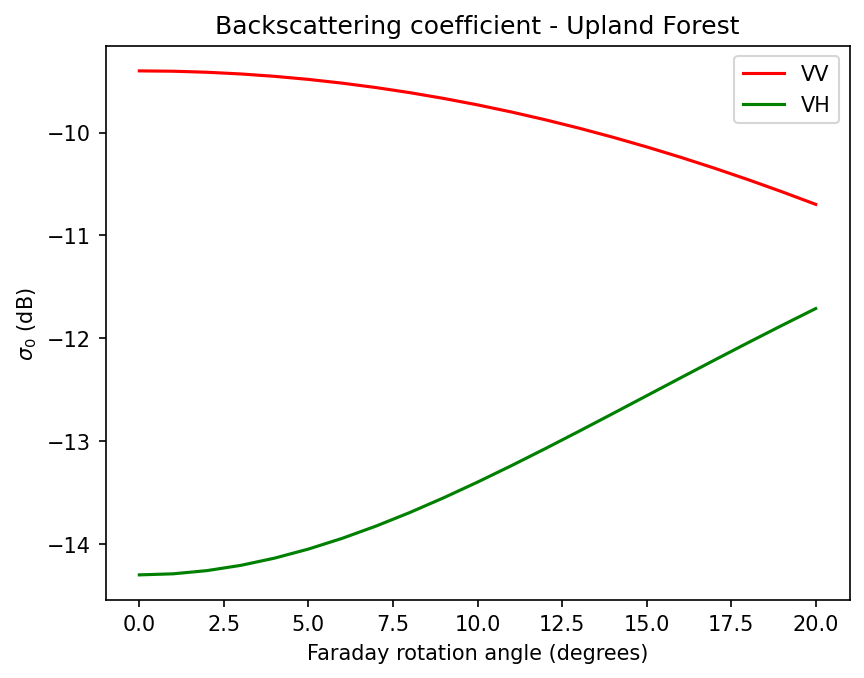
\includegraphics[width=0.32\textwidth]{Figures/pol/FR_bacskcatter_Upland Forest.png}
 & 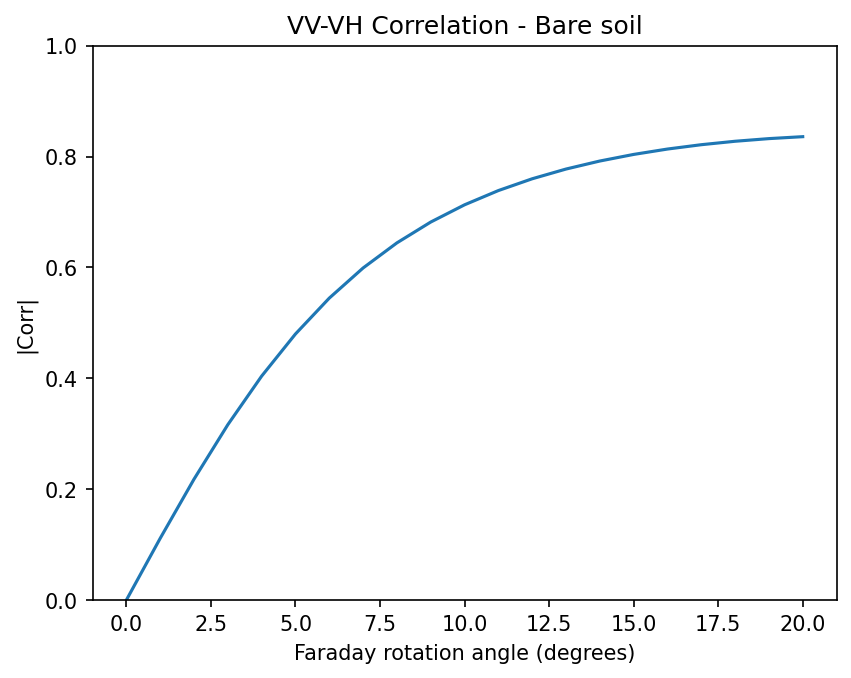
\includegraphics[width=0.32\textwidth]{Figures/pol/FR_VV-VH_Correlation_Bare soil.png}
 &
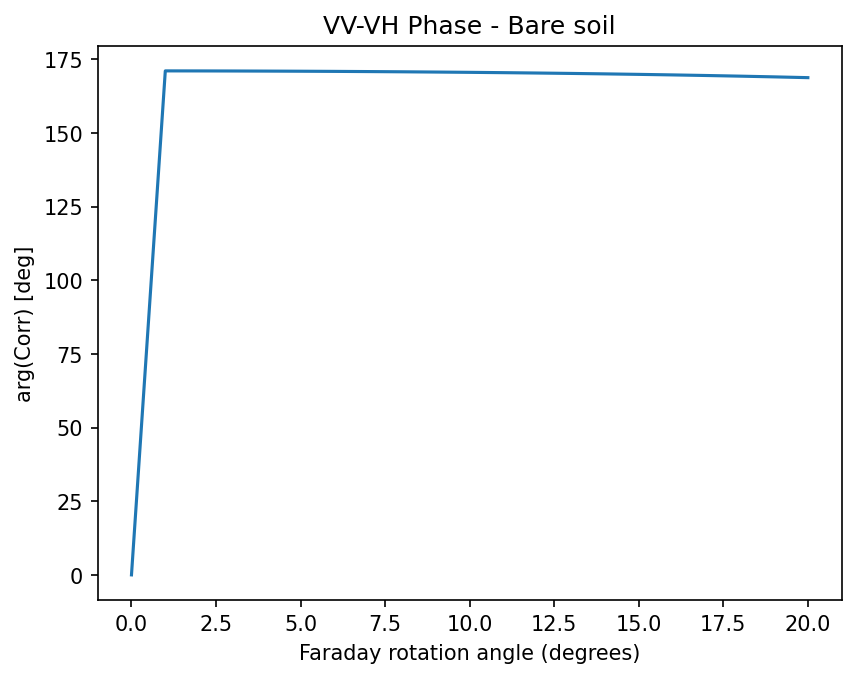
\includegraphics[width=0.32\textwidth]{Figures/pol/FR_VV-VH_Phase_Bare soil.png} \\
(a) & (b) &
(c) 
\end{tabular}
\caption{Effect of \acs{fr} upon the dual-pol response of forest. (a) Backscattering coefficients, (b) Correlation between channels, (c) Phase between channels.}
\label{fig:pol_fr_dualpol_forest}
\end{figure}

The backscattering coefficient at the copolar channel (VV) decreases as the rotation angle increases. This decrease is almost negligible for angles lower than 5~degrees, and reaches 1 to 2~dB at the extreme cases (rotation angle equal to 20~degrees). At the cross-polar channel (VH), the backscattering coefficient increases proportionally to the \acs{fr} angle, reaching a bias of 7~dB for bare soil (\autoref{fig:pol_fr_dualpol_baresoil}a) and 3~dB for forest (\autoref{fig:pol_fr_dualpol_forest}a). 

Due to the cross-talk induced by \acs{fr}, the most severely affected polarimetric variable is the correlation between channels. A scene characterised by null correlation exhibits a rapidly increasing correlation as a consequence of \acs{fr}. For instance, it reaches 0.5 at a rotation angle of 5~degrees, and saturates at around 0.8 for rotation angles above 15~degrees.

The phase difference between the two channels is not defined when the correlation between channels is null. However, it takes a value close to 180~degrees as soon as the  \acs{fr} make the correlation depart from zero.

In the same vein, Figure 3 shows the false colour RGB composites of a SAOCOM scene over Naples when \acs{fr} is injected into the data and no correction is applied. For this purpose, the backscattering level of HH is assumed equal to VV and the correlation between HH and VV is assumed to be 0.5 with zero phase. This has been applied as a constant for the whole scene, but these values could be changed in a more sophisticated way, e.g. as a function of the land cover type.

\begin{figure}[ht!]
\centering
\begin{tabular}{cc}
No FR & 5 degrees \\
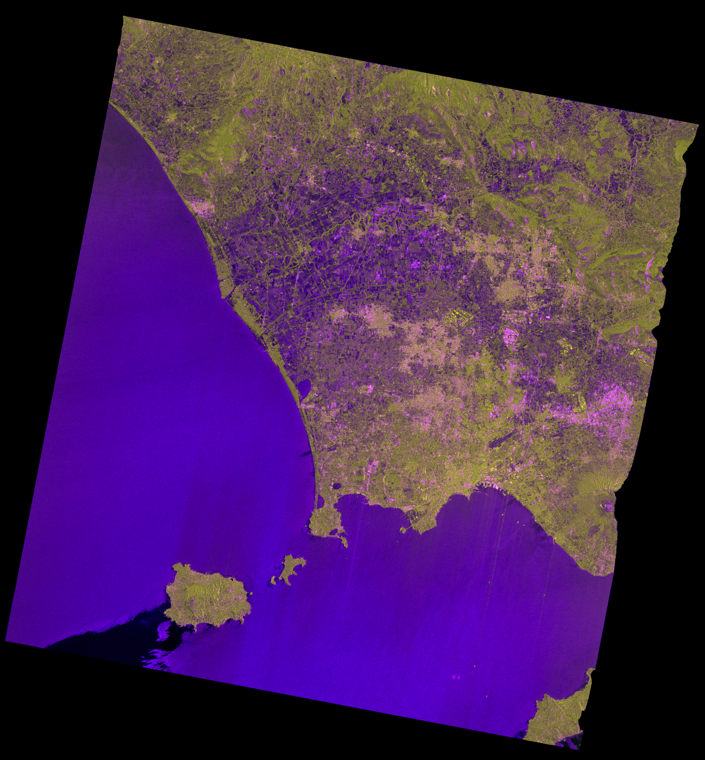
\includegraphics[width=0.45\textwidth]{Figures/pol/SAOCOM_RGB_noFR.png}
 & 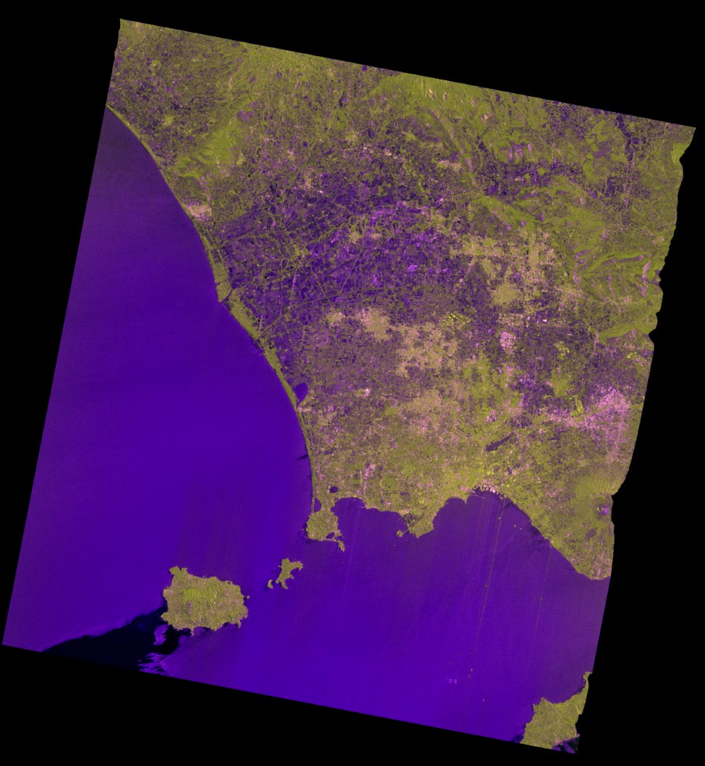
\includegraphics[width=0.45\textwidth]{Figures/pol/SAOCOM_RGB_FR_5deg.png}
 \\
10 degrees & 20 degrees \\
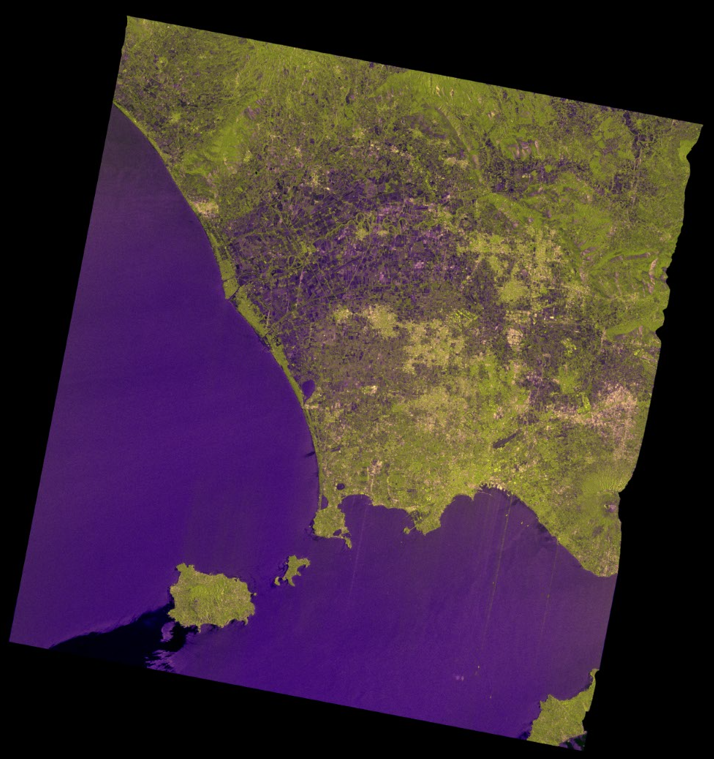
\includegraphics[width=0.45\textwidth]{Figures/pol/SAOCOM_RGB_FR_10deg.png}
 & 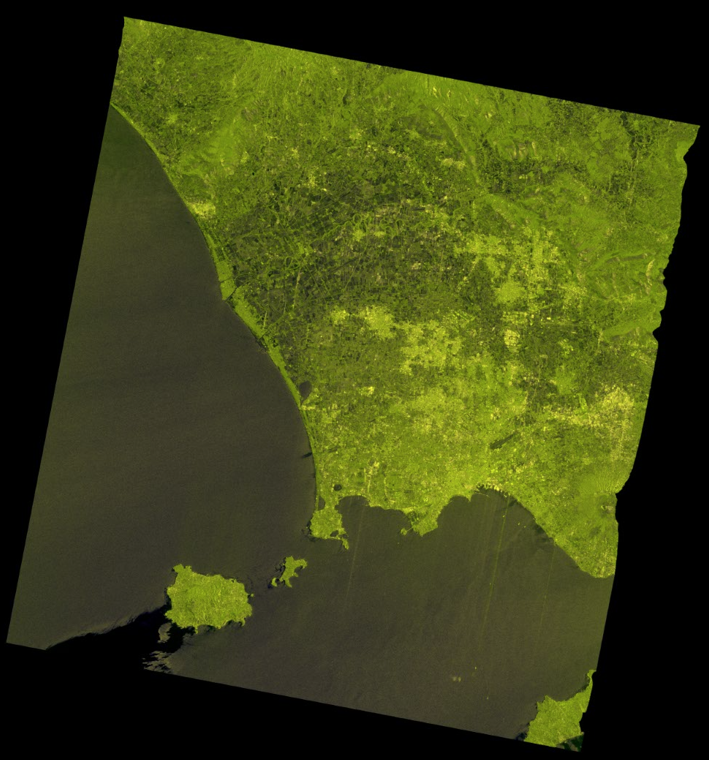
\includegraphics[width=0.45\textwidth]{Figures/pol/SAOCOM_RGB_FR_20deg.png}

\end{tabular}
\caption{RGB false colour composite of a SAOCOM dual-pol image over Naples (DSC/S4). Channels: R: VV, G: VH: B: VV/VH. The original image (top left) is compared with other three cases in which different \acs{fr} angles were injected (5, 10 and 20~degrees). The backscattering level of HH is assumed equal to VV and the correlation between HH and VV is assumed to be 0.5 with zero phase, and both are assumed constant over the whole scene.}
\label{fig:pol_FR_RGB}
\end{figure}

The visual aspect of the RGB composite when the \acs{fr} angle  is 5~degrees is very similar to the case without \acs{fr}, as the VV backscattering coefficient is almost unaltered and the VH one is only increased by less than 2~dB. A \acs{fr} angle of 10~degrees is more noticeable in this image: the sea becomes purple instead of blue, and all areas originally represented in pink colour (corresponding to buildings and urban land cover) become yellowish. In the most extreme case (\acs{fr} angle equal to 20~degrees) the polarimetric information is lost, and the resulting image is all shown in the same green hue, with its brightness defined by the span (backscactered power).

A summary of the results of a simple correction approach for dual-pol data, using real measurements of \acs{tec}, and the expected impact of \acs{fr} FR for ROSE-L were described in Chapter~6 of \citep{Hajnsek2019}.
Assuming certain knowledge on the scene (land cover and scattering properties), which can be obtained from other quad-pol L-band images of other sensors (e.g. ALOS-PALSAR and NISAR), and by using an external measure of \acs{tec}, it is possible to approximately correct the effect of FR on dual-pol data. These approaches  could be readily implemented, and they could be tested using quad-pol data as a reference. If no correction is applied, external \acs{tec} values could be used to estimate the \acs{fr} rotation angle and produce an auxiliary map with the expected impact of \acs{fr} (or a mask map if binarized). 
